\chapter{TRABALHOS RELACIONADOS}\label{cha:Trabalhos_relacionados}

O desenvolvimento de plataformas robóticas móveis para fins educacionais, de pesquisa e industriais tem ganhado destaque nas últimas décadas, em virtude da crescente popularização de microcontroladores de baixo custo e do amadurecimento de frameworks de software abertos como o \textit{Robot Operating System} (ROS). Essa combinação tem permitido a criação de sistemas robóticos cada vez mais acessíveis, modulares e escaláveis, abrindo espaço para experimentação e inovação em diferentes contextos.

No âmbito acadêmico, diversos trabalhos vêm propondo a utilização de robôs móveis como ferramentas didáticas para o ensino de conceitos de automação, eletrônica e programação embarcada. \citeonline{vilanova2022aeronave} propôs o desenvolvimento de uma plataforma robótica aérea baseada na aeronave DJI® Ryze Tello (Figura \ref{fig:tello}) no Robot Operating System (ROS 2) voltada para práticas educacionais de robótica móvel em laboratório, conforme previsto na Proposta Pedagógica Curricular (PPC) do curso de Engenharia Mecânica do Instituto Federal do Piauí (IFPI). O autor defendeu a utilização de uma estrutura robótica experimental como recurso didático para aplicação dos conteúdos de controle, automação e sistemas embarcados, integrando sensores, atuadores e comunicação em rede em um ambiente real de aprendizagem. A pesquisa evidenciou que o uso do ROS 2 em contextos educacionais favorece a compreensão dos princípios de arquitetura modular e comunicação entre nós, permitindo que o estudante vivencie o ciclo completo de desenvolvimento robótico — da programação embarcada à análise de desempenho do sistema.

\begin{figure}[!ht]
    \Caption{\label{fig:tello} DJI ® Ryze Tello Combo Boost.}
    \centering
    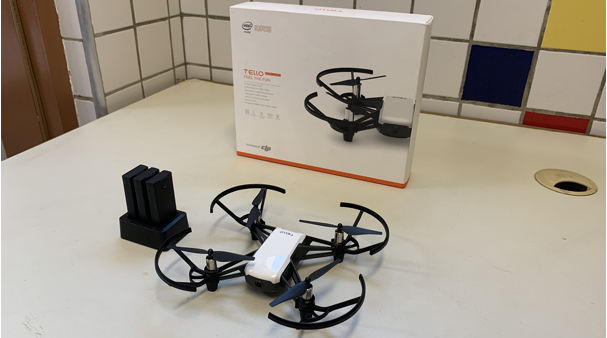
\includegraphics[scale=0.8]{figuras/tello.png}
    \legend{\Fonte{\cite{vilanova2022aeronave}.}}
\end{figure}

Em consonância com essa proposta, \citeonline{Dantas_2022} desenvolveu uma plataforma robótica móvel adaptada a partir do aspirador Roomba® 614 iRobot , visando, primordialmente, o ensino de robótica para o curso de Engenharia Mecânica do IFPI. O autor estruturou o projeto em torno do microcontrolador ESP32 , o qual, mediante a utilização do framework micro-ROS , viabiliza a integração direta com o ambiente ROS 2. Ademais, o trabalho introduziu uma base impressa em 3D projetada para acoplar sensores adicionais , garantindo, assim, a versatilidade necessária para diversas práticas experimentais em laboratório.

\begin{figure}[!ht]
    \caption{\label{fig:roomba_dantas} Roomba 614 iRobot montado com estrutura 3D impressa}
    \centering
    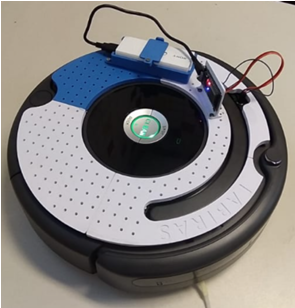
\includegraphics[width=0.5\linewidth]{figuras/roomba_dantas.png}
    \legend{\Fonte{\cite{Dantas_2022}}}
\end{figure}